\documentclass{report}
\usepackage{amsmath}
\usepackage{amsfonts}
\usepackage{graphicx}
\usepackage[utf8x]{inputenc} 
\title{Machine Learning lecture notes}
\author{Khoa Hoang Viet \thanks{based on Andrew Ng's Machine Learning course in coursera.org}}
\date{\today}
\begin{document}
\section{Neural Networks}
\subsection{Model Representation I}
Let's examine how we will represent a hypothesis function using neural networks. At a very simple level, neurons are basically computational units that take inputs (\textbf{dendrites}) as electrical inputs (called "spikes") that are channeled to outputs (\textbf{axons}). 

In our model, our dendrites are like the input features $x_1\cdots x_n$, and the output is the result of our hypothesis function. In this model our $x_0$ input node is sometimes called the "bias unit." It is always equal to 1. In neural networks, we use the same logistic function as in classification, $\frac{1}{1 + e^{-\theta^Tx}}$, yet we sometimes call it a sigmoid (logistic) \textbf{activation} function. In this situation, our "theta" parameters are sometimes called "weights".

Visually, a simplistic representation looks like:
$$\begin{bmatrix}x_0 \\ x_1 \\ x_2 \\ 
\end{bmatrix}
\rightarrow
\begin{bmatrix}\ \ \ \\ \end{bmatrix}
\rightarrow h_\theta(x)$$
Our input nodes (layer 1), also known as the "input layer", go into another node (layer 2), which finally outputs the hypothesis function, known as the "output layer".

We can have intermediate layers of nodes between the input and output layers called the "hidden layers."

In this example, we label these intermediate or "hidden" layer nodes $a^2_0 \cdots a^2_n$ and call them "activation units."
\begin{align*}
	& a_i^{(j)} = \text{"activation" of unit $i$ in layer $j$} \\
	& \Theta^{(j)} = \text{matrix of weights control function mapping from layer $j$ to layer $j+1$}
\end{align*}

If we had one hidden layer, it would look like:
$$\begin{bmatrix}x_0 \\ x_1 \\ x_2 \\ x_3\end{bmatrix}
\rightarrow
\begin{bmatrix}a_1^{(2)} \\ a_2^{(2)} \\ a_3^{(2)} \\ \end{bmatrix}
\rightarrow h_\theta(x)$$

The values for each of the "activation" nodes is obtained as follows:
\begin{align*} 
	a_1^{(2)} = g(\Theta_{10}^{(1)}x_0 + \Theta_{11}^{(1)}x_1 + \Theta_{12}^{(1)}x_2 + \Theta_{13}^{(1)}x_3) \\ 
	a_2^{(2)} = g(\Theta_{20}^{(1)}x_0 + \Theta_{21}^{(1)}x_1 + \Theta_{22}^{(1)}x_2 + \Theta_{23}^{(1)}x_3) \\ 
	a_3^{(2)} = g(\Theta_{30}^{(1)}x_0 + \Theta_{31}^{(1)}x_1 + \Theta_{32}^{(1)}x_2 + \Theta_{33}^{(1)}x_3) \\ 
	h_\Theta(x) = a_1^{(3)} = g(\Theta_{10}^{(2)}a_0^{(2)} + \Theta_{11}^{(2)}a_1^{(2)} + \Theta_{12}^{(2)}a_2^{(2)} + \Theta_{13}^{(2)}a_3^{(2)}) \\ 
\end{align*}

This is saying that we compute our activation nodes by using a 3×4 matrix of parameters. We apply each row of the parameters to our inputs to obtain the value for one activation node. Our hypothesis output is the logistic function applied to the sum of the values of our activation nodes, which have been multiplied by yet another parameter matrix $\Theta^{(2)}$ containing the weights for our second layer of nodes.

Each layer gets its own matrix of weights, $\Theta^{(j)}$.

The dimensions of these matrices of weights is determined as follows:

"If network has $s_j$ units in layer $j$ and $s_{j+1}$ units in layer $j+1$, then $\Theta^{(j)}$ will be of dimension $s_{j+1} \times (s_j + 1)$."

The +1 comes from the addition in $\Theta^{(j)}$ of the "bias nodes," $x_0$ and $\Theta_0^{(j)}$. In other words the output nodes will not include the bias nodes while the inputs will. The following image summarizes our model representation:\\
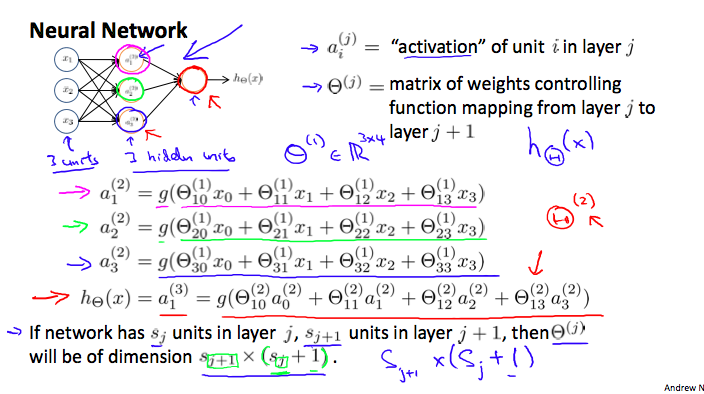
\includegraphics[width=\textwidth]{model_representation.png}
 
Example: If layer 1 has 2 input nodes and layer 2 has 4 activation nodes. Dimension of $\Theta^{(1)}$ is going to be 4×3 where $s_j = 2$ and $s_{j+1} = 4$, so $s_{j+1} \times (s_j + 1) = 4 \times 3$.

\end{document}